\begin{figure}[h]
\begin{center}
%%\fbox{
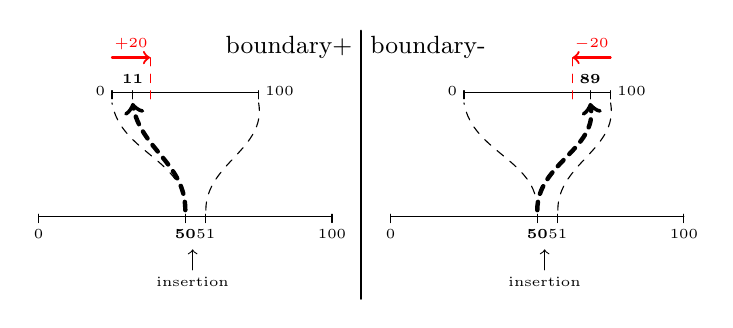
\begin{tikzpicture}[scale=0.745,cap=round]
\small

%% Titles
  \draw (5.5,82pt) -- node[anchor=east]{boundary+} (5.5,82pt);
  \draw (5.5,82pt) -- node[anchor=west]{boundary-} (5.5,82pt);

\tiny
%% Boundary +
  \draw [<-] (2.625,-16pt)--( 2.625, -26pt)  node[anchor=north] {insertion};

  \draw  (1.25,60pt)-- ( 3.75, 60pt);
  \draw  (0,0)-- (5, 0);
  
  \draw [dashed] (2.5,3pt) to[out=90,in=280] (1.25,55pt);
  \draw [->,ultra thick,dashed] (2.5,3pt) to[out=90,in=280] (1.6,55pt);
  \draw [dashed] (2.85,3pt) to[out=90,in=280] (3.75,55pt);  
  
  \draw [->,thick,color=red] (1.25,77pt) -- node[anchor=south]{$+20$}
  (1.9,77pt);
  \draw [dashed, color=red] (1.9,77pt) -- (1.9,57pt);


  \draw (0,1pt) -- (0,-3pt) node[anchor=north] {0};
  \draw (5,1pt) -- (5,-3pt) node[anchor=north] {$100$};
  \draw (1.25,57pt) -- (1.25,61pt) node[anchor=east] {0};
  \draw (1.6,57pt) -- (1.6,61pt) node[anchor=south] {\textbf{11}};
  \draw (3.75,57pt) -- (3.75,61pt) node[anchor=west] {$100$};
  \draw (2.5,1pt) -- (2.5,-3pt) node[anchor=north] {\textbf{50}};
  \draw (2.85,1pt) -- (2.85,-3pt) node[anchor=north] {$51$};


%% Delimitation
  \draw [thick] (5.5,-40pt) -- (5.5, 90pt);

%% Boundary -
  \draw [<-] (8.625,-16pt)--( 8.625, -26pt)  node[anchor=north] {insertion};

  \draw  (7.25,60pt)-- ( 9.75, 60pt);
  \draw  (6,0)-- (11, 0);
  
  \draw [dashed] (8.5,3pt) to[out=90,in=280] (7.25,55pt);
  \draw [->,ultra thick,dashed] (8.5,3pt) to[out=90,in=280] (9.4,55pt);
  \draw [dashed] (8.85,3pt) to[out=90,in=280] (9.75,55pt);  

  \draw [->,thick,color=red] (9.75,77pt) -- node[anchor=south]{$-20$}
  (9.1,77pt);
  \draw [dashed, color=red] (9.1,77pt) -- (9.1,57pt);
  
  \draw (6,1pt) -- (6,-3pt) node[anchor=north] {0};
  \draw (11,1pt) -- (11,-3pt) node[anchor=north] {$100$};
  \draw (7.25,57pt) -- (7.25,61pt) node[anchor=east] {0};
  \draw (9.4,57pt) -- (9.4,61pt) node[anchor=south] {\textbf{89}};
  \draw (9.75,57pt) -- (9.75,61pt) node[anchor=west] {$100$};
  \draw (8.5,1pt) -- (8.5,-3pt) node[anchor=north] {\textbf{50}};
  \draw (8.85,1pt) -- (8.85,-3pt) node[anchor=north] {$51$};


\end{tikzpicture}
%%}

\caption{Choice of the digit part of identifiers in \emph{boundary+} (left) and
  \emph{boundary-} (right). In both case: constant base set to $100$,
  boundary value set to $20$ and the random number is $11$. The results are
  $[50.11]$ (\emph{boundary+}) and $[50.89]$ (\emph{boundary-}).}
\label{img:positionchoice}
\end{center}
\end{figure}
